\documentclass[11pt]{article}
\usepackage{times}
\usepackage[dvips]{graphicx}
\usepackage{latexsym,fullpage,amsmath,listings}
%\usepackage{latexsym,fullpage,times}
\usepackage{float,array}
\usepackage[colorlinks]{hyperref}

\begin{document}

\begin{center}
{\Large ME/IE/CS 558}\\
\vspace{12pt}
{\large Final Project: Shape Processing}\\
\vspace{12pt}
{\em Due May 4, 2018}
\end{center}

{\bf For all assignments:}
{\em Unless specifically indicated,  you are free to use any
publicly available sources: papers, books, programs, online
material, etc. -- as long as you clearly indicate and attribute
the origin of the information.}

\vspace{12pt}
The goal of this assignment is to gain experience with tasks in polygonal shape processing:  (1) construction, (2) validation,  (3) querying, (4) triangulation, and (5) computation of its medial axis.   Specific requirements for each task are described below. 

\begin{enumerate}
\item {\em Construction.}
Your first challenge is to construct the polygonal approximation of a shape $S$ defined by an inequality $f(x,y) \ge 0.$   More specifically,  given an expression $f(x,y)$ and a size parameter $h$,  your program needs to  construct  a piecewise linear approximation (a connected sequence of line segments)  of the boundary $\partial S$ defined by  $f(x,y) = 0$, such that the length of every segment is  $\le h$.\footnote{The set $f(x,y) = 0$ is sometimes called a level set of $f$, and its computation is sometimes called contouring.} Discuss how this is achieved by your construction in the analysis report. 

\item {\em Validation.}  Generally speaking,  there is no guarantee that $f(x,y)=0$ is not empty or that it corresponds to the boundary of a valid shape $S_p$.  For the purpose of this assignment, we shall assume that a shape $S_p$ is valid if it is a simple polygon.  Describe and implement all tests necessary to determine if the collection of line segments bounds a simple polygon $S_p$.  

\item {\em Querying.}  In case the computed shape $S_p$ is a simple polygon, design and implement an efficient point membership test and distance computation for an arbitrary point $p$.   Point membership test should return in/on/out result;  distance query should return the shortest distance from point $p$ to the polygon's boundary.

\item {\em Triangulation}
Design and implement an algorithm of your choice to compute triangulation of the polygon $S_p$.  The running time of the algorithm should not be worse than $O(n^2)$.

\item {\em Medial Axis}
Design and implement an algorithm to compute (either exactly or approximately) the medial axis of the polygon $S_p$.  The running time of the algorithm should not be worse than $O(n^2)$. 

\end{enumerate}



\paragraph { Analysis (50 points)}

The analysis portion of the project should discuss all mathematical assumptions, data structures, and algorithms in the implementation of the above tasks.  Provide running time analysis of your algorithms using the usual $O()$ notation.   In the construction task, discuss any limitations or guarantees provided by your algorithm. (For example,  can you miss some important features?  what happens to sharp corners of $S$?  etc.)   If any of your algorithms are approximate  (for example, medial axis computation),  clearly discuss the quality of approximation.  





\paragraph{ Implementation \& Testing (50 points)}

\begin{enumerate}

\item 
Implement the program to produce graphic outputs showing the computed piecewise linear approximation of $f \ge 0$ (including its interior), triangulation and medial axis respectively.

\item The input to the program is string  specifying the function as a Python expression,   such as    "5*x**3 - 17.3 * y**2 + sin(x*y)" , etc.  and a real number specifying the value of the size parameter $h$. 
The expressions may be evaluated in Python using eval() function.  

\item
Test your program on variety of functions.  Wolfram is a good source for variety of such functions
\href{http://mathworld.wolfram.com}{http://mathworld.wolfram.com}

\item
During grading, there are two input files. The expression file specifies the implicit expression, axis limits and $h$. The points file defines several points for point membership check. 

The format of \textbf{expression file} is
\begin{lstlisting}
expression
xmin, xmax, ymin, ymax
h
\end{lstlisting}
You can assume the expression defines a function $f(x, y)$. And the level set ($f(x, y) = 0$) is within the domain $[x_{min}, x_{max}] \times [y_{min}, y_{max}]$. 

The format of \textbf{points file} (you can assume the delimiter is tab) is
\begin{lstlisting}
x1	y1
x2	y2
...
xn	yn
\end{lstlisting}

your program will be called from command line as
\begin{lstlisting}
>> python shape_processing.py <expression_file> <points_file>
\end{lstlisting}

For the below expression file
\begin{lstlisting}
-x**2/4 - y**2 + 9
-7, 7, -4, 4
1
\end{lstlisting}
and points file
\begin{lstlisting}
0	0
100	0
\end{lstlisting}

A valid solution includes plotting (see Figure \ref{fig:construction} - \ref{fig:medial}) and the below command line output. 

\begin{lstlisting}
The constructed boundary is a simple polygon.
Point membership check and minimum distance are listed below
(0, 0) : in, 2.961293
(100, 0): out, 94.062987
\end{lstlisting}
If the constructed boundary is not a simple polygon, you program should output ``the constructed boundary is not a simple polygon'' and exit.
\begin{figure}[H]
  \centering
  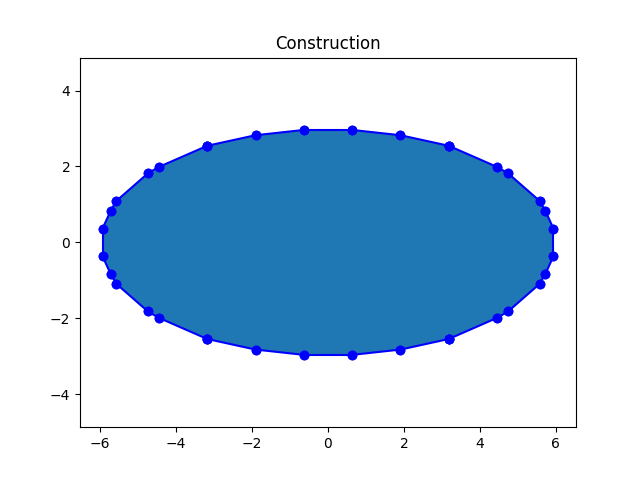
\includegraphics[scale=0.4]{construction.png}
  \caption{Construction (boundary and interior defined by $f > 0$)}
  \label{fig:construction}
\end{figure}

\begin{figure}[H]
  \centering
  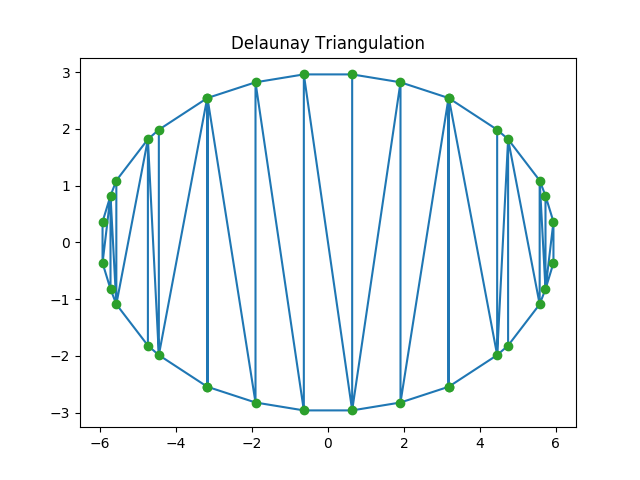
\includegraphics[scale=0.4]{delaunay_triangulation.png}
  \caption{Delaunay triangulation}
  \label{fig:triangulation}
\end{figure}

\begin{figure}[H]
  \centering
  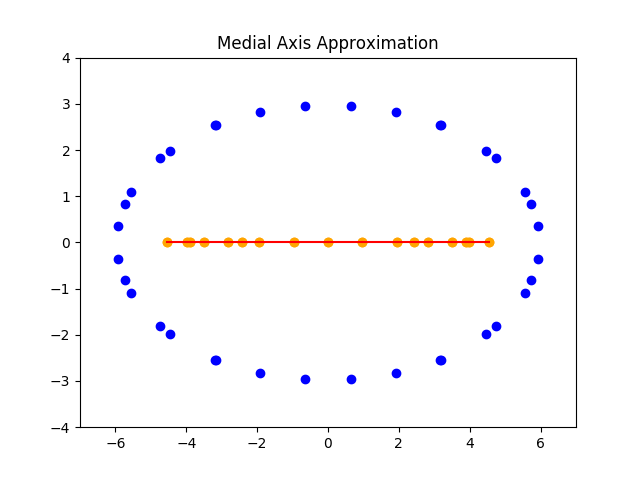
\includegraphics[scale=0.4]{medial_axis.png}
  \caption{Medial Axis Approximation}
  \label{fig:medial}
\end{figure}

\item Please also provide four other python files which are used for partial credit grading.\\

The first python file is called ``reconstruction.py'' which is for step 1 and step 2. It will be called from command line as below.
\begin{lstlisting}
>> python reconstruction.py <expression_file>
\end{lstlisting}
It produces graphic outputs showing the computed piecewise linear approximation of $f \ge 0$ (including its interior) and prints whether the boundary is a simple polygon or not to command line.

The second python file is called ``pmc.py'' which is for step 3. It will be called from command line as below.
\begin{lstlisting}
>> python pmc.py <polygon_file> <points_file>
\end{lstlisting}
Polygon file is represented by its vertices in ccw orientation. For example a unit square is represented by
\begin{lstlisting}
0	0
1	0
1	1
0	1
\end{lstlisting}
Its output is the point membership check and minimum distance results. 

The third python file is called ``triangulation.py'' which is for step 4. It will be called from command line as below.
\begin{lstlisting}
>> python triangulation.py <polygon_file>
\end{lstlisting}
It plots a triangulation of the polygon.

The third python file is called ``medial\_axis.py'' which is for step 5. It will be called from command line as below.
\begin{lstlisting}
>> python medial_axis.py <polygon_file>
\end{lstlisting}
It plots the approximated medial axis of the polygon.


\end{enumerate}

\paragraph {Extra Credit} (up to 15 points)
\begin{enumerate}
\item
Extend your program to work on more general types of polygons defined by $f(x,y) \ge 0$ (e.g., with holes, disconnected, etc.)
\item 
Improve your point membership test and distance computation algorithm to perform better than $O(n)$ time (with pre-processing).  
\item
Modify your triangulation program to compute Delaunay triangulation of the polygon. 
\item 
Design and implement $O(n)$ algorithm to compute convex hull of the polygon. 

\end{enumerate}



\section*{Deliverables}

Please use the course website to submit a single  zip  named   FirstName\_LastName\_Project.zip
The zip archive should contain:  (1) the analysis portion of the assignment,  (2)  the documented python source file, and (3) a PDF readme file  specfying the instructions for running the code.  It should also include at least 1 sample run with input and output,  and specify any specific dependencies or requirements of your code.  


\end{document} 
